% !TEX root = ../../ausarbeitung.tex
\subsection{Applying Bayes' Theorem to Particle Decays and Branching Ratios}
\label{sec:analysis:bayes}
We examine a newly discovered particle which was found to be able to decay in two different ways. 
This means there are two different decay channels, α and β. 
The probability \( \falpha \) for decay α to happen is called the \quotedef{branching ratio}.
We can recognize that each decay is a Bernoulli trial, because of two reasons. 
First, there are exactly two outcomes: it can \emph{either} go to channel α \emph{or} to channel β. 
Second, the probabilities of a decay going to either channel are fixed.
Therefore, the probabilities for one decay are
\begin{subequations}
\begin{gather}
    P(\symup{α}) = \falpha, \\
    P(\symup{β}) = 1 - \falpha.
\end{gather}
\end{subequations}

When the number of trials \( N \) is fixed, a series of \emph{statistically independent} Bernoulli trials is called a Bernoulli process.
A Bernoulli process is described by the binomial distribution,
\begin{equation}
    \label{eq:bayes:binomial_distribution}
    P(N, k, \falpha) = \binom{N}{k} \, \falpha^k \, (1 - \falpha)^{N - k}.
\end{equation}
Here, \( N \) is the total number of decays, \( k \) is the number of \quotedef{successes}, i.e. the number of decays to channel α, and \( \falpha \) is the probability of a decay going to the α channel.
Therefore, with a fixed number \( N \) of observed decays, the number of decays to one of the channels (e.g. α) follows a binomial distribution.

\subsubsection{Bayes' Theorem}
\label{sec:analysis:bayes:bayes_theorem}
As explained previously, Bayes' Theorem tells us how to update our beliefs about a parameter of a distribution when we get new information from measurements.
In this case the model is a Bernoulli process, described by the binomial distribution in \autoref{eq:bayes:binomial_distribution}.
The binomial distribution is dependent on the probability \( p \), which is our parameter.

We start with some notion of what this parameter might be.
This is codified in the prior probability distribution, \( \pi(p) \).
In the Bayesian sense the function gives the level of confidence (probability) that a certain value for \( p \) is correct.

If we make a set of observations \( \vec{k} \), we can then calculate the likelihood \( L(\vec{k} | \falpha) \) of these observations given our model,
\begin{equation}
    L(\vec{k} | \falpha) = \prod_{k_i \in \vec{k}} P(k_i, \falpha),
    \label{eq:bayes_theorem:likelihood_definition}
\end{equation}
where each \( k_i \) is the number of successes in a number of trials \( N \).

Finally, we can calculate the probability of the parameter taking on a certain value given our observations.
\begin{gather}
    % do we want to insert P(k | f) from above explicitly?
    P(\falpha|\vec{k}) = \frac{L(\vec{k}|\falpha) \, P(\falpha)}{\int L(\vec{k}|\falpha) \, P(\falpha) \, \mathrm{d}\falpha}
    \label{eq:bayes:posterior}
\end{gather}

\autoref{eq:bayes:posterior} shows the \emph{Posterior Probability Distribution} for this experiment. As was explained before, this gives us a probability distribution over the possible values of the parameter \( \falpha \). This lets us estimate what the true value of the original system is.

\subsubsection{Calculating the Posterior Probability Distribution}

Assuming a small number of measurements we can explicitly calculate the posterior distribution of \( \falpha \).

If a single decay was measured and it went to \( \alpha \), the likelihood is simply \( L(\alpha | \falpha) = \falpha \). Because we have no reason to weight our distribution before the first piece of data, the prior distribution will be flat and limited to the interval \( [0, 1] \), because probabilities of discrete events must be between \num{0} and \num{1}. Therefore, \( \pi(\falpha)=1 \forall \falpha\in[0,1] \) and the posterior is:
\begin{gather}
    P(\falpha|\alpha) = \frac{\falpha \cdot 1}{\int _0 ^1 \falpha \cdot 1 \, \mathrm{d}\falpha} \\
    P(\falpha|\alpha) = 2 \falpha
    \label{eq:bayes_theorem:posterior_1_decay}
\end{gather}

If another measurement is made, we can use \autoref{eq:bayes_theorem:posterior_1_decay} as the new prior and calculate the likelihood using \autoref{eq:bayes_theorem:likelihood_definition}.

This approach of starting with a prior, making observations, then calculating the posterior to become the next prior is called \quotedef{updating beliefs}.
It is very logical and useful.
However, often the necessary integrals are only numerically integrable, which means lots of time and computing power are needed to find the result.
Here the concept of a "conjugate prior" comes in handy.

The general idea is to find a function specified by some set of \quotedef{hyperparameters} such that for the given type of experiment the calculated posterior will also be a function of the same form, just with different values for the hyperparameters.

For the Bernoulli process, which is described by a binomial distribution, this conjugate prior is called the beta distribution.
It has the form
\begin{gather}
    \pi(p) = \frac{p^{\alpha - 1} (1 - p)^{\beta - 1}}{\Beta(\alpha, \beta)}, \quad p \in [0,1]
\end{gather}
where \( \alpha \) and \( \beta \) are the hyperparameters and \( \Beta \) is the beta function. The beta function normalizes the beta distribution.

While the calculations of the posterior are analytically solvable for a small number of measurements we implement the more robust method using conjugate priors. The beta distribution is implemented in the \texttt{scipy.stats} package, which we will use in our implementation of the calculations.

For a single measurement, our calculation will show that this method is equivalent to the analytic function \( P(\falpha|\alpha) = 2 \falpha \).

Using the conjugate prior method, we graph the prior and posterior probability distributions of \( \falpha \) in \autoref{fig:bayes_theorem:prior_posterior_one_alpha_decay}.

\begin{figure}[htbp]
    \centering
    % Prior and posterior of observing one alpha decay
    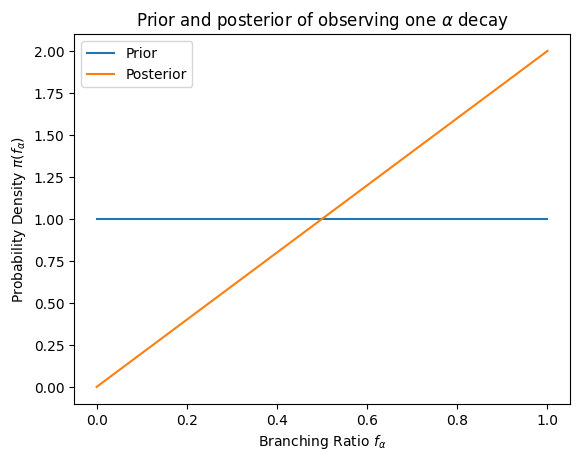
\includegraphics[width=0.5\textwidth]{Graphs/Bayes/one_decay.png}
    \caption{Prior and Posterior Probability Distribution of \( \falpha \), Given One \( \alpha \) Decay}
    \label{fig:bayes_theorem:prior_posterior_one_alpha_decay}
\end{figure}

Now we are given five total measurements: \( (\alpha, \beta, \alpha, \alpha, \beta) \).

We now set the previous result as the new prior and calculate the new posteriors after one more of these measurements, until we have used all measurements to inform the posterior.

% We make use of the fact that calculating the posterior twice, once after event \( x_1 = (n_1, k_1) \) and once after event \( x_2 = (n_2, k_2) \), gives the same result as calculating the posterior after event \( x = x_1 + x_2 = (n_1 + n_2, k_1 + k_2) \).

To see the evolution of our knowledge about the parameter \( \falpha \), in \autoref{fig:bayes_theorem:posteriors_2_to_5} we graph the posteriors after each new data point is added.

\begin{figure}[htbp]
    \centering
    
\includegraphics[width=0.5\textwidth]{pGraphs/Bayes/multiple_decays.png}
    \caption{Evolution of Posterior Distributions after Multiple Observations}
    \label{fig:bayes_theorem:posteriors_2_to_5}
\end{figure}

Because of our robust implementation for calculating posteriors, we can now use the same code to calculate the posterior after a large number of decays. In this case, we are given a total of \( n = \num{100} \) decays, with \num{58} going to \( \alpha \). The posterior is given in \autoref{fig:bayes_theorem:posterior_100_decays}.

\begin{figure}[htbp]
    \centering
    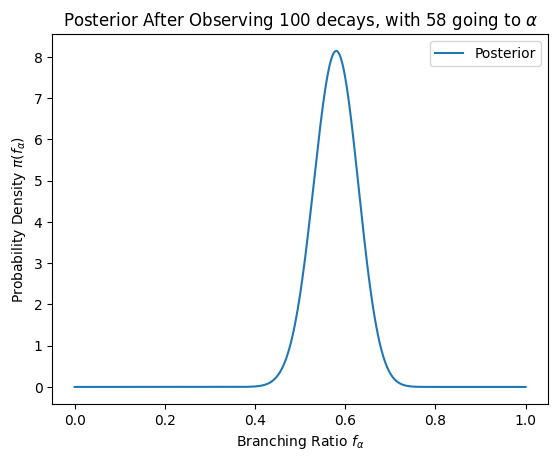
\includegraphics[width=0.5\textwidth]{Graphs/Bayes/100_decays.png}
    \caption{Posterior Probability Distribution of \( \falpha \), Given \num{100} Data Points}
    \label{fig:bayes_theorem:posterior_100_decays}
\end{figure}